\documentclass[../main.tex]{subfiles}

\begin{document}
    \chapter{Background}\label{chap:background}

    This chapter provides a brief overview of the problems addressed in this work, as well as the main
    technologies upon which our approach is designed.
    Section~\ref{sec:domainadapt} is a description of the domain adaptation problem in the context
    of machine learning, in which the main challenges of the field are highlighted.
    Section~\ref{sec:deeplearning} is an introduction to the basics of Deep Learning,
    a branch of machine learning concerned with the study and the design of Artificial Neural Network (ANN) models.
    This section draws heavily on~\cite{Goodfellow-et-al-2016}.

    \section{Domain Adaptation}\label{sec:domainadapt}

    \paragraph{Introduction}
    At the core of the majority of machine learning (ML) techniques, there is the optimization of some
    error (also called loss) function $L(y, \hat{y}; \theta)$, that is a function of the reference output $y$, the output
    of the model $\hat{y}$, and the parameters of the model $\theta$.
    \newline
    Although machine learning draws a lot from optimization methods, there is a seemingly small but profound difference
    between the two. In sheer mathematical optimization, we have full access to the function we want to minimize (or maximize),
    while in ML this is not true. In particular, in ML we have access to only a subset of the input-output relationship,
    and we minimize the error function over this sample in the hope that doing this will also minimize the overall error function
    (which we don't know).
    $$ L_{sample}(y, \hat{y}; \theta) = \frac{1}{N} \sum_{i = 1}^{N} L(y_{i}, \hat{y_{i}}; \theta) $$
    In this framework, what we really care about is \textbf{generalization}, that is the ability of an algorithm to obtain a good
    performance on samples it has never seen before (such samples are called \textit{test sets}), according to some performance measure $P$.
    \paragraph{The i.i.d.\ assumption}
    A typical assumption done in machine learning settings is that the \textit{training set}
    $( X_{train}, Y_{train} )$\footnote{Here we are focusing only to supervised settings, but the domain adaptation problem
    can be defined also for unsupervised ones} (the sample used to minimize $L$) and the \textit{test set} $( X_{test}, Y_{test} )$
    (the sample used to evaluate generalization) are \textbf{i.i.d.}, that is, they are independently sampled from the same
    underlying distribution $P(X, Y)$. The majority of algorithms operate under this assumption, which is usually a fairly good
    approximation. But the are cases in which this assumption does not hold, and this causes a significant drop in performance between
    training and testing.
    \paragraph{Motivation}
    Domain Adaptation~\cite{domain-adaptation-review} consists in the design of algorithms that work even when the i.i.d.\
    assumption does not hold, i.e.\ when the distribution from which training samples are drawn is different from the
    one at testing time.
    Domain adaptation has a slightly different terminology with respect to classical ML\@. In particular, the training distribution
    is called the \textit{source domain} $D_{S}$, while the testing distribution is called the \textit{target domain} $D_{T}$.
    Typically, we assume that the source data is abundant and labeled, while the target data is only partially labeled, or not at all
    labeled. Clearly, this is the most interesting setting because solving this problem would allow us to leverage data sets for
    which we have lots of labeled data, and at the same time obtain good performance on the data sets we were interested in the first
    place, but which often have few labeled data. This setting goes under the name of \textit{Unsupervised} Domain Adaptation. If instead
    we assume that the target is partially of fully labeled, we talking about \textit{Semi-Supervised} or \textit{Supervised} Domain
    Adaptation respectively. This work in particular focuses exclusively on the unsupervised setting, which is clearly harder.
    \paragraph{Domain Adaptation}
    In machine learning, the joint distribution of data and labels $P(X, Y)$ is, of course, unknown. In domain adaptation,
    we call the joint distribution of the source domain $ P_{s}(X, Y) $, while $ P_{t}(X, Y) $ is the joint distribution of
    the target domain. The i.i.d.\ assumption consists in a assuming that $ P_{s}(X, Y) = P_{t}(X, Y) = P(X, Y) $.
    In Domain Adaptation instead, we have $ P_{s}(X, Y) \neq P_{t}(X, Y) $. We can visually see what are the implications
    of this in figure~\ref{fig:AD-tsne}.
    \newline
    The source data is drawn i.i.d.\ from the source distribution, while the target data is drawn i.i.d.\ from the marginal
    over $X$ of the target distribution:
    \begin{align*}
        S = (X_{s}, Y_{s}) \sim D_{S} = P_{s}(X, Y) \\
        T = (X_{t}) \sim D_{y} = P_{t}(X)
    \end{align*}
    The goal is to build a classifier $f : X \rightarrow Y$ capable of making correct predictions about the target labels $Y_{t}$:
    $$ \text{maximize}   P(Y_{t} = \hat{Y_{t}}) $$
    Where $\hat{Y_{t}} = f(X_{t})$ are the labels predicted by the classifier and $Y_{t}$ are the true target labels, which we
    don't know.

    \begin{figure}
        \centering{}
    	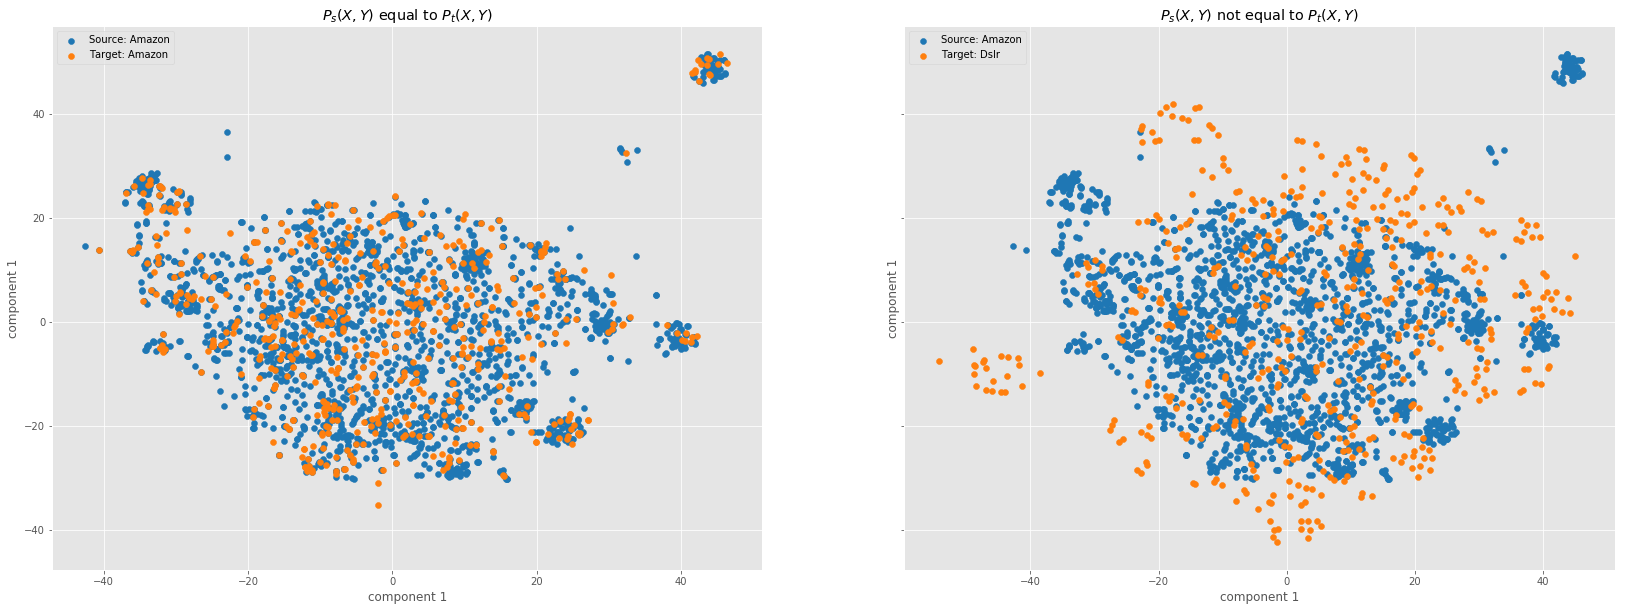
\includegraphics[width=\linewidth]{img/AD-alexnet-tsne.png}
        \caption{t-SNE~\cite{tsne} visualization of the features extracted from the Office dataset using AlexNet. When the source
        and the target distribution are the same (left), a classifier trained on the source data generalizes very well to the target
        data. When the i.i.d.\ assumption does not hold (right), generalization performance will be poor.}\label{fig:AD-tsne}
	\end{figure}

    \section{Deep Learning}\label{sec:deeplearning}

    \paragraph{Introduction}
    Artificial Intelligence (AI) technologies have to deal with the fact that current machines are very different from humans.
    In fact, it can be said that they are the opposite. Many tasks that require effort and reasoning for a human to accomplish,
    such as chess, are pretty easy for machines, because such problems can be encoded into a set of formal rules that machines
    are particularly suited to deal with. Conversely, other kinds of tasks that a human doesn't even need to think about
    are tremendously difficult for machines. These are the tasks we find so easy to perform that we don't even manage to explain how
    we achieve them. Encorporating the intuition and common sense that humans give for granted is one of the holy grails of AI.\@
    \paragraph{History}
    At first, it was believed that intelligent behavior could be achieved by hard-coding knowledge into the system by means
    of some formal language. Reasoning would then be achieved through the use of inference rules, such as Modus Ponens.
    These were the so-called \textbf{Expert Systems}.
    It was soon evident that the number of formal rules needed for intelligent behavior exceeds by several orders of magnitude
    the number of rules one could possibly write by hand.
    \newline
    This led to a major shift from deductive systems to inductive ones, where the machine itself \textit{learns} to extract
    knowledge from data. By seeing a lot of input-output examples in the form $y = f(x)$ it would figure out the relationship $f$ itself.
    This was the beginning of \textbf{Machine Learning} (ML). In classical ML the input representation is still hand-crafted though.
    For instance, a classical ML image classification algorithm does not take in input the raw pixels of the image, but some other
    representation created by an ad-hoc procedure. This was a drawback because the majority of efforts went into the
    \textit{feature engineering} process itself, and in many cases this is more an art than a science.
    \newline
    The natural evolution of this is to not only let the program learn the input-output relation $y = f(x)$,
    but also the input representation as well. That is, the algorithm learns both a suitable representation of the input $\phi(x)$, and then
    the relationship between this representation and the output $y = f(\phi(x))$. This research field is called \textbf{Representation Learning}.
    \newline
    \textbf{Deep Learning} is an extension of representation learning. The machine learns multiple levels of representations
    in a hierarchical fashion, where more complex concepts are built on top of simpler ones.
    Deep Learning is nowadays behind many state-of-the-art techniques in many research fields, like computer vision and speech recognition,
    and many believes it to be one of the most promising ways to reach human level artificial intelligence someday.
    \newline
    In the following, we will provide a very concise introduction to the main concepts of deep learning. In particular, we will cover only a
    tiny subset of the whole field: \textit{feed-forward (convolutional) neural networks} for \textit{supervised learning} (classification).
	Thus, the setting is the typical one for classification problems: we have a \textit{data set} of $n$ samples, of which the i-th sample
	is $(X_{i} \in \mathbb{R}^{1 \times n}, Y_{i} \in \{1, 2, \ldots, C\})$, where $X_{i}$ is a row vector of numerical features, and $Y_{i}$
	is the class label for sample $i$. The task is to come up with a model capable of predicting the correct class label $Y^{'}$ for a previously
	unseen instance $X^{'}$.

    \subsection{Feed-Forward Neural Networks}
    The Feed-Forward Network can be thought of as a general framework in which different layers of processing units are stacked on top
    of each other. Each layer implements a function that takes in input the output of the previous layer.\footnote{Note that also the input and
    the output of the network are considered layers}. A single layer can be viewed either as implementing a vector valued function or
    as a set of parallel processing units, each of which takes in input the outputs of the units in the previous layer and performs some
    sort of computation. The name neural networks stem from the fact that these models are loosely inspired by how the human brain works,
    and in this regards, the parallel processing units in each layer perform a role analogous to that of neurons in the brain.
    The classical example of a feed-forward network architecture is the MultiLayer-Perceptron (MLP)~\cite{mlp}, in which
    each layer implements an affine mapping of the input followed by an element-wise non-linear function:

    \begin{equation}
        h = \sigma(Wx + b)
    \end{equation}

    Where $x \in \mathbb{R}^{m \times n}$ is the layer's input, $h \in \mathbb{R}^{m \times p}$ is the output,
    $\sigma$ is the non-linearity (called the \textit{activation function}) and
    $W \in \mathbb{R}^{n \times p}, b \in \mathbb{R}^{p}$ are the layer's parameters.
    The parameters $W$ are called the \textit{weights}; in MLPs there is a different weight for each pair of input-output units.
    The intercept of the affine mapping $b$ is called the \textit{bias}, because it represents the output of the layer when
    the input is zero. Regarding $\sigma$, there exists many non-linearities in the deep learning literature, some of the most popular are the
    \textit{sigmoid or logistic} function, the \textit{hyperbolic tangent (TanH)} and the \textit{rectifier linear unit (ReLU)}:

    \begin{equation}
        Sigmoid(x) = \frac{1}{1 + e^{-x}}, TanH(x) = \frac{e^{x} - e^{-x}}{e^{x} + e^{-x}}, ReLU(x) = \max(0, x)
    \end{equation}

    The layer $h = \sigma(Wx + b)$ described above can be thought of as a way of stretching and squashing space in order to project
    the input onto a new space in which it is linearly separable, that is, there exists a hyperplane separating the different classes.
    In the following depiction we can see such a layer in action:

    \begin{figure}[h!]
        \centering
        \begin{subfigure}{\textwidth}
            \centering
        	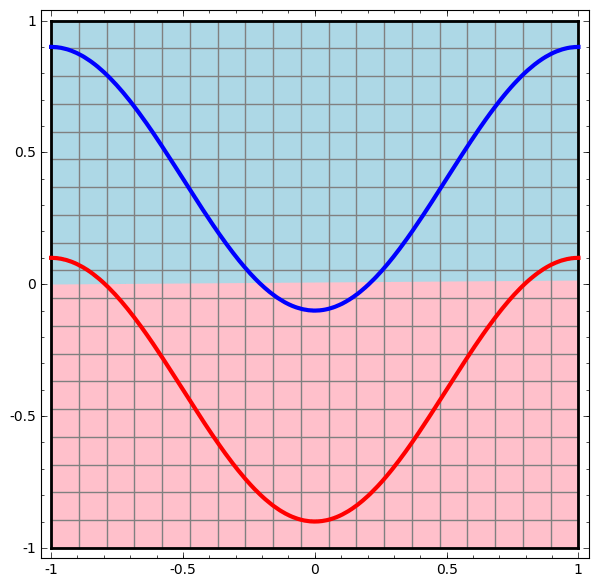
\includegraphics[width=.4\linewidth]{img/non-linearly-separable.png}\label{fig:nonlinearsep}
        \end{subfigure}
        \begin{subfigure}{\textwidth}
            \centering
        	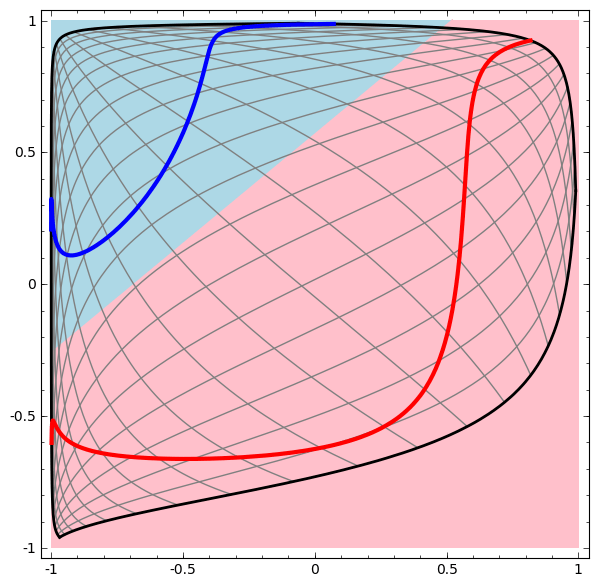
\includegraphics[width=.4\linewidth]{img/linearly-separable.png}\label{fig:linearsep}
        \end{subfigure}
        \footcaption{The original data (left) is not linearly separable, that is, there does not exists a hyperplane capable of
            separating the red curve from the blue curve. The transformation $h = \sigma(Wx + b)$ project the input x into a new space
        (right) where it's easy to find a separating hyperplane.}\label{fig:linear-layer-viz}
	\end{figure}

    \footnotetext{Images taken from: \url{http://colah.github.io/posts/2014-03-NN-Manifolds-Topology/}}

    When we stack a number of such layers one on top of the other, we have a deep network. In particular, the input-output mapping defined by
    a MultiLayer-Perceptron with $n$ layers is recursively defined as:

    \begin{equation}
        \hat{y} = W_{n}(\sigma(W_{n-1}(\sigma(W_{n-2}(\ldots W_{1} x + b_{1} \ldots)) + b_{n-2})) + b_{n-1}) + b_{n} 
    \end{equation}

    With $W_{1}, b_{1}$ denoting the parameters of the first layer and $W_{n}, b_{n}$ the parameters of the last layer. The dimension of the
    first layers is constrained to be $(m, \cdot)$, with $m$ number of inputs, while the dimension of the last layer is constrained to be
    $(\cdot, c)$, with $c$ number of classes. The dimensions of all the other layers are hyper-parameters of the model that the designer
    of the architecture can arbitrarily chose. The number of layers $n$ is also a hyper-parameter.
    \newline
    The output vector $\hat{y}$ has one entry for each class, and it can be thought of as the scores the network assigns to different classes.
    Since this vector can assume arbitrary values, it is typically followed by a function which converts the raw class scores into a
    probability distribution over classes, that is that normalizes the scores so that they sum to one.
    The most popular function used in the deep learning literature is the \textbf{softmax} function:

    \begin{equation}
        softmax(z) = \left[ \frac{e^{z_{1}}}{\sum_{i = 1}^{c} e^{z_{i}}} , \ldots , \frac{e^{z_{c}}}{\sum_{i = 1}^{c} e^{z_{i}}} \right], z = \left[ z_{1}, \ldots ,z_{c}  \right]
    \end{equation}

    Thus, the complete input-output mapping of the MLP is:

    \begin{equation} \label{eq:MLPequation}
        \hat{y} = softmax(W_{n}(\sigma(W_{n-1}(\ldots W_{1} x + b_{1} \ldots)) + b_{n-1}) + b_{n})
    \end{equation}

    Now that we've defined our model, we need two more things: a definition of error and a procedure to learn from such errors.

    \paragraph{The Loss Function}
    The first thing to note is that the output of the model is a vector with $c$ entries, one for each class. So we need to define the
    reference value $y$ also as a vector with $c$ entries. This is done by using the so-called \textit{one-hot-encoding}, that is, class
    $i$ is represented by a vector in which the $i$-th position is 1 and the other $c - 1$ positions are 0.\footnote{For instance, in a ten class
    classification problem, class 6 would be represented as $y_{6} = \left[ 0, 0, 0, 0, 0, 1, 0, 0, 0, 0 \right] $.} Having both
    the model output $\hat{y}$ and the reference value $y$, we can define the loss function. The most popular choice for classification
    tasks in deep learning is the \textbf{cross-entropy} loss function, defined as:

    \begin{equation}
        L(y, \hat{y}; \theta) = - \sum_{i = 1}^{c} y_{i} \log(\hat{y_{i}}) + (1 - y_{i})\log(1 - \hat{y_{i}})
    \end{equation}

    It is easy to see that for all the entries for which $y_{i} = 0$, only the second term contributes to the loss, and for the entry
    for which $y_{i} = 1$ (the true label), only the first term contributes to the loss. The previous equation is the cross-entropy loss for a single
    input sample. In deep learning (and more generally in machine learning), the loss is usually averaged over a number of samples,
    called a \textit{mini-batch}. In this case, the loss becomes:

    \begin{equation}
        L(y, \hat{y}; \theta) = - \frac{1}{N} \sum_{i = 1}^{N} \sum_{j = 1}^{c} \left[ y_{i, j} \log(\hat{y_{i, j}}) + (1 - y_{i, j})\log(1 - \hat{y_{i, j}})  \right]
    \end{equation}

    Now we know how to compute the model's errors with respect to reference values. The last thing to cover is the design of a learning
    procedure, that is how to modify the model's parameters in order to reduce future errors.

    \paragraph{The Learning Algorithm}
    In Deep Learning, the most popular technique for minimizing the loss function is \textbf{gradient descent}. The basic idea
    is that the gradient of the loss function with respect to the model parameters gives us the direction of maximum increase
    of the loss. Hence, by updating the parameters in the opposite direction, we are effectively minimizing the error.
    Formally, the learning rule is the following:

    \begin{equation}
        \theta^{k+1} = \theta^{k} - \alpha \nabla L(y, \hat{y}; \theta)
    \end{equation}

    Where $\alpha$ is a hyper-parameter of the algorithm that controls the step size in the direction of steepest descent. It is called the
    \textbf{learning rate} in the literature. This parameter is of fundamental importance in the optimization procedure, as its value often
    makes the difference between convergence and divergence of the minimization process. The previous was the most basic version of gradient
    descent. Other techniques have been developed in recent years to overcome the major limitations of this scheme. The momentum~\cite{momentum}
    method provides a sort of short-term memory of recent updates to the optimizer and it helps smoothing the trajectory of minimization and
    improving speed of convergence. More recent methods like Adam~\cite{adam} are more sophisticated, as they employs per-parameter
	adaptive learning rates.
	\newline
    Now we know how to modify the network's parameters
    in order to minimize the loss function, but how do we compute the gradients? It turns out there is a very computationally efficient
    algorithm which allows us to compute the partial derivatives of the loss with respect to the model's parameters. This algorithm is called
    \textbf{backpropagation}.

    \paragraph{The BackPropagation Algorithm}
    The BackPropagation algorithm~\cite{backprop} computes partial derivatives in a feed-forward neural network\footnote{Although this
	technique is mainly used in the context of neural networks optimization, the algorithm is general and can be used to differentiate
	arbitrary functions}.
	\newline
	The reference value $y$ is defined with respect to the output layer of the network, so it is easy to compute the gradient of this
	layer. Hidden layers instead do not have target values, so their gradient cannot be computed directly. But we know that hidden layers
	influence the output of the last layer, because they provide the representation on top of which the output layer is built. BackPropagation
	uses this fact to recursively compute the gradients starting from the output layer and going backwards to the first hidden layer. Hence the
	name BackPropagation. In particular, BackPropagation cleverly uses the chain rule of calculus to compute the partial derivatives
	in previous layers. The chain rule of calculus basically states that if we have a nested function
    $ z = f(y) = f(g(x)) $, the derivative of z w.r.t.\ x is equal to:
    $$ \frac{dz}{dx}  = \frac{dz}{dy} \frac{dy}{dx} $$
    This is similar to the structure of equation~\ref{eq:MLPequation}. The full learning procedure of a MultiLayer-Perceptron is showed in Algorithm~\ref{algbackpropagation}.

    \begin{algorithm}
    \caption{MultiLayer-Perceptron learning algorithm. \newline
    The \textbf{forward} function computes the output of the network given input $x$: $\hat{y} = f(x; \theta)$.
    The \textbf{backward} function computes the gradients of the loss function with respect to the model parameters. It starts with the gradient of the output layer, and then it propagates it backwards.
    The \textbf{update} function updates the parameters of the network according to the gradient descent update rule.
    The three functions must always be called in the exact order: forward \rightarrow{} backward \rightarrow{} update}\label{algbackpropagation}
    \begin{algorithmic}[1]

        \Require{$net$, the network}
        \Require{$(x, y)$, (input, target output)}

        \Function{forward}{$net, x, y$}
            \State{$h[0] = x$}                               \Comment{h is a tensor holding the outputs of all layers}
            \For{$k = 1, \ldots, d$}                         \Comment{d is the depth (number of layers)}
                \State{$a[k] = net.W[k] h[k-1] + net.b[k]$}
                \State{$h[k] = \sigma(a[k])$}
                \State{$net.a[k] = a[k]$}
            \EndFor{}
            \State{$\hat{y} = h[l]$}
            \State{$J(\hat{y}, y; \theta) = L(\hat{y}, y; \theta) + \lambda \Omega(\theta)$ \Comment{$\lambda \Omega(\theta)$} is the regularization term}
            \State{\textbf{return} $(\hat{y}, J(\hat{y}, y; \theta))$}
        \EndFunction{}

        \Function{backward}{$net, y$}
            \State{$g = \nabla_{\hat{y}} J(\hat{y}, y; \theta)$}     \Comment{gradient of the output layer}
            \For{$k = l, \ldots, 1$}                                 \Comment{from output to input}
                \State{$g = \nabla_{a[k]} J = g \odot f'(net.a[k])$} \Comment{gradient before the non-linearity}
                \State{$net.gradB[k] = \nabla_{net.b[k]} J = g + \lambda \nabla_{net.b[k]} \Omega(\theta)$}
                \State{$net.gradW[k] = \nabla_{net.W[k]} J = g h^{(k-1)T} + \lambda \nabla_{net.W[k]} \Omega(\theta)$}
                \State{$g = \nabla_{h^{(k-1)}} J = {net.W[k]}^{T} g$}  \Comment{propagate the gradients below}
            \EndFor{}
        \EndFunction{}

        \Function{update}{net}
            \For{$k = l, \ldots, 1$}
                \State{$net.b[k] = net.b[k] - \alpha \cdot net.gradB[k]$}
                \State{$net.W[k] = net.W[k] - \alpha \cdot net.gradW[k]$}
            \EndFor{}
        \EndFunction{}

    \end{algorithmic}
    \end{algorithm}

    \subsection{Convolutional Neural Networks}
    As we saw in the previous section, in the standard feed-forward net each layer is composed by an affine mapping followed by some non-linearity.
    But this is not the only way in which layers can be designed. There exists several kinds of feed-forward architectures, and in this section
    we will see what is arguably the most popular and successful example of specialization: the Convolutional Neural Network (CNN).
    \newline
    CNNs are a specialization of the feed-forward network, particularly suited to work with data in which spatial information is important, like
    time series in one dimension and images in two dimensions. If we have to train a standard feed-forward net to classify images, the first
    thing we would do is to transform the 2D image into a 1D vector by concatenating together all the pixel values. By doing this we are
    clearly losing the spatial information relating the pixel to one another. Conv nets instead are capable of fully exploit the spatial
    correlations between pixels.
    \newline
    More formally, a Convolutional Neural Network is a feed-forward network in which at least one layer uses the convolution operation.

    \subsubsection{The Convolution Operation}
    The convolution operation employed in deep learning (also called \textit{cross correlation}) is a linear operation.
    In the case of two dimensional data, in particular images, the output at pixel $(i, j)$ is a weighted linear combination
    of a neighborhood around $(i, j)$. The set of weights is called the \textit{kernel}. It is easy to understand this operation
    by looking at picture~\ref{fig:convolution-op}:

    \begin{figure}[h!]
        \centering
    	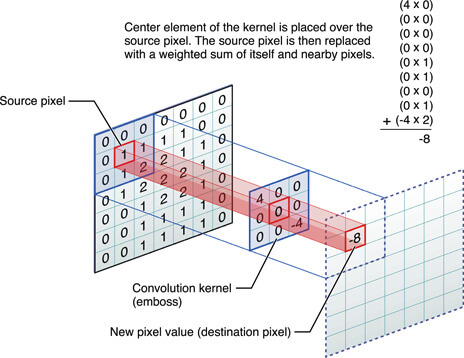
\includegraphics[width=.8\linewidth]{img/convolution-op.png}
        \footcaption{The Convolution operation}\label{fig:convolution-op}
	\end{figure}

    \footnotetext{Image taken from: \url{https://developer.apple.com/library/content/documentation/Performance/Conceptual/vImage/ConvolutionOperations/ConvolutionOperations.html}}

    More formally, the convolution operation for pixel $(i, j)$ is defined by the following:
    \begin{equation}
        F(i, j) = (I \ast K)(i, j) = \sum_{w} \sum_{h} I(i + w, j + h) K(w, h)
    \end{equation}
    Where $I$ is the input image, $K$ is the convolution kernel, and $F$ is the output, also called \textit{feature map}. The full
    feature map is defined by applying the previous operation for $i = 1, \ldots, w$ and for $j = 1, \ldots, h$, that is, the kernel
    is a window that slides over the entire image, computing the weighted combination at each pixel location. The kernel can be thought
    of as a specialized filter, which produces high responses to certain features of the input. For instance, a filter can produce a
    high response when it sees a vertical edge, or a blotch, and a low response in any other case.

    \subsubsection{Learning the kernels}
    The exists many techniques based on convolution and kernel to compute edges or other features in the input image (Ex: Sobel operator).
    The main difference with those approaches is that in Conv nets, the filters are not hand-crafted, but instead the network \textbf{learns}
    the values of the filters. In particular, in each convolutional layer, several kernels are computed in parallel, with each one specializing
    in the detection of a different feature. As a consequence of the hierarchical nature of deep learning, filters in low level layers specialize
    in the detection of low-level features such as edges and blobs, while high-level filters specialize in the detection of more high-level features,
    such as faces and animals.

    \begin{figure}[h!]
    	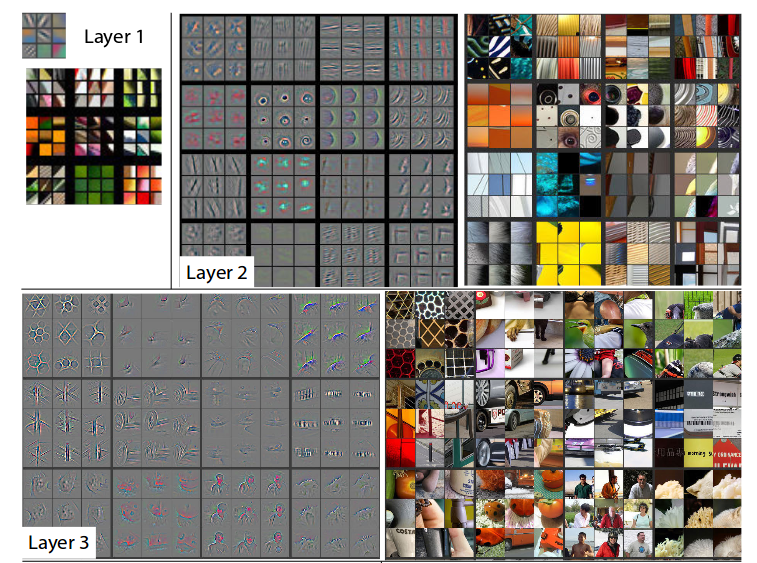
\includegraphics[width=\linewidth]{img/learned-conv-filters.png}
        \caption{Visualizing Conv net filters, taken from~\cite{zeiler13}}\label{fig:conv-filters}
	\end{figure}

    In the next section we will see the other building block of CNNs, the \textit{pooling} operation.

    \subsubsection{Pooling in Convolutional Networks}
    In CNNs, a convolutional layer is usually followed by a pooling layer, that is a way of performing dimensionality reduction
    and improving the network overall robustness to input transformation. In particular, a pooling layer replaces the output of the
    network at pixel location $(i, j)$ with a summary statistics of nearby pixels. Many statistics are employed in the deep learning
    literature (refs). The most popular is arguably Max Pooling (ref), in which the summary statistic is simply that maximum value.
    The following depition shows how Max Pooling works:

    \begin{figure}[h!]
        \centering
    	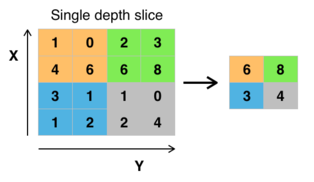
\includegraphics[width=.6\linewidth]{img/max-pooling.png}
        \caption{Max Pooling operation.}\label{fig:max-pooling}
	\end{figure}

    It has been shown (ref) that the spatial pooling operation improves invariance to small translations in the input, i.e.\ if the
    input image is translated some pixels to the left or right, the output is still the same. This is a nice property to have when
    dealing with images, because we aren't usually interested in knowing precisely where a feature, we are only concerned with whether
    the feature is actually present or not.

    \subsubsection{Advantages of Convolutional Networks}
    Convolutional Neural Networks have some unique features that make them particularly efficient, from both a computational and a
    computer vision perspective. The three main advantages of CNNs with respect to standard feed-forward networks are:
    \begin{itemize}
        \item \textbf{Sparse Interactions}: the feed-forward net is composed of affine layers $Wx + b$ where there is a different
            parameter for each pair of input-output units. Thus, each layer of the net has a number of parameters that is $O(m \times n)$,
            where $m$ is the number of input units and $n$ the number of output units. CNNs instead has a number of parameters that
            is $O(k \times w \times h)$, where $k$ is the number of filters and $w, h$ are respectively width and height of each filter.
            Since kernels are typically much smaller that the input, CNNs can have less parameters by orders of magnitude.

        \item \textbf{Parameter Sharing}: As we said in the previous point, feed-forward nets have a different parameter for each pair
            of input-output units. In CNNs instead, each kernel is re-used over the entire input.
            This can be viewed as a parameter sharing technique, in which we have $m$ kernels with the constraint that they have to
            have the same parameters. Of course, in practice, we have only one kernel that is used as a sliding window over the input,
            but thinking of it as a use of parameter sharing can give more insights into how CNNs work.

        \item \textbf{Translation equivariance}: The convolution operation is naturally equivariant to translation, i.e.\ if the input is
            translated by a small amount of pixels to the left or right, the output is translated by the same amount.  This is clearly a
            desirable property when analizying images. This operation is not naturally invariant to other input transformations such as 
            scaling and rotation, but CNNs as a whole can achieve such properties with appropriate mechanisms.
    \end{itemize}

\end{document}
